\documentclass{article}
\usepackage{amsmath}
\usepackage{mathtools}
\usepackage{graphicx}% Include figure files
\usepackage{bm}% bold math
\usepackage{verbatim}
\usepackage{color}
\usepackage[colorlinks=true,linkcolor=blue,citecolor=cyan]{hyperref}
\usepackage{appendix}


\newcommand{\warning}[1]{{\textsf{{\textcolor{red}{{[#1]}{}}}}}}
\let\vec\mathbf

\begin{document}

\title{A cumulant analysis of free energy decompositions}
\author{Jason A. Wagoner and Justin L. MacCallum}

\date{ \today}

\maketitle

\begin{abstract}
Stuff...
\end{abstract}


\section{Introduction}

\subsection{Free energy decompositions offer insight into driving forces and mechanisms.}

We are interested in decomposing a single free energy calculation into meaningful contributions from various components of the Hamiltonian. 
This is an attractive prospect; free energy components could be used to understand the driving forces underlying the free energy and to make predictions about how the free energy will change if different parts of the system are changed. For example, in a protein-protein binding calculation with N total residues, labeled $i \in \left[1, \ldots,N\right]$, we may wish to estimate the contribution of each residue $i$ to binding. Doing this rigorously requires $N+1$ separate binding free energy calculations, which is often computationally prohibitive. Instead, free energy decompositions potentially allow us to estimate the contribution of each residue from a single simulation.

Unfortunately, these free energy decompositions can be problematic. Obtaining a decomposition may be easy, but obtaining a meaningful or interpretable decomposition is difficult. The central issue is that, aside from idealized cases, free energy changes are \textit{non-additive}. The available phase space of the system depends strongly on the Hamiltonian. Changes to one component of the Hamiltonian can completely change the available phase space, thus strongly influencing the values of other components. So, it is often unclear how the non-additive parts are allocated to the different free energy components. This also leads to a second problem, that free energy decompositions are \textit{path dependent}. Although the total free energy is a state function, the non-additive components (and, therefore, the free energy components themselves) depend on the alchemical path taken in the calculation. These combined issues make it unclear exactly how these free energy components should be interpreted; i.e., what is their physical meaning, and how can they be used to make predictions? 

Mark and Van Gunsteren have used these arguments to conclude that free energy decompositions are too problematic and should not be used~\cite{Smith:1994tn,Mark:1994un}. Karplus, Sharp, and others have argued that in many cases the couplings may be small and thus free energy components still provide useful information if interpreted carefully~\cite{Boresch:1994jj,Brady:1995dz,Boresch:1995ux,Archontis:1996ef}. 

Despite these major caveats, there is a long history of using free energy decompositions to gain semi-quantitative understanding of important molecular systems. [refs here]. Free energy decompositions are also used in chemical engineering~\cite{Dixit:2011cl,Gu:2017ec}. [more refs if we want] [also cite Huggins]

Here, we analyze free energy decompositions using a cumulant expansion. The cumulant expansion grants intuition into how the different components contribute to the overall enthalpy and entropy of the system and into the origin of free energy couplings. The cumulant expansion also gives a solid footing from which to build free energy decompositions as it explicitly reveals how the coupled terms are partitioned into the different free energy components. 

We use the cumulant expansion to show that all previous free energy decompositions result in components that are not true free energies--they do not correspond to differences in thermodynamic potential between two states, and they cannot be measured experimentally. We present a new decomposition that does in fact give real free energies that are easy to interpret and that directly correspond to experimental measurements.  This decomposition contains a series of univariate and multivariate components, where each univariate component $i$ corresponds to the total free energy less the free energy were that component $i$ of the Hamiltonian removed from the system. Similarly, a multivariate component $ij$ gives a coupling term analogous to those calculated in double mutant experiments. These free energy components are more difficult to calculate exactly, but we show that reliable estimates can be obtained by including and truncating the cumulant expansion in the free energy calculation. 

\section{Theory}


%%%%%%%%%
%%%%%%%%%
%%%%%%%%%
\subsection{Background of free energy calculations, thermodynamic integration, and cumulant expansions}
%%%%%%%%%
%%%%%%%%%
%%%%%%%%%

Consider a system with Hamiltonian $H(x, \lambda) = H_0 (x) + H_1(x, \lambda) + H_2(x, \lambda)$ parameterized by a control parameter $\lambda$. The components $H_1$ and  $H_2$ each depend on $\lambda$ in some arbitrary way, while $H_0$ does not.  These Hamiltonian components may correspond to a decomposition of energy terms (Lennard Jones, charged interactions, etc.) or to a decomposition across different degrees of freedom (per-residue interactions, for example). For ease of presentation, we largely focus on this case of two components, but our results readily generalize to an arbitrary number of Hamiltonian components. Hereafter, to simplify notation, we omit the $x$-dependence of the Hamiltonian and its components.

The excess free energy compared to an ideal gas is:
\begin{equation}\label{eq:dA}
A(\lambda) = -\beta^{-1} \left[ 
	\ln \int e^{-\beta H(\lambda)} dx - 
	\ln \int dx
\right],
\end{equation}
where $\beta=1/k_BT$, $k_B$ is Boltzmann's constant, and $T$ is the absolute temperature.

%%%%%%%%%
%%%%%%%%%
\subsubsection{Free energy changes can be calculated by thermodynamic integration}
%%%%%%%%%
%%%%%%%%%

We can compute the free energy difference between the states $\lambda=0$ and $\lambda=1$ using thermodynamic integration:
\begin{align}
\Delta A =&  A(1) - A(0) \nonumber\\
               =& \int_0^1 \frac{\partial }{\partial \lambda}  A(\lambda) d \lambda \nonumber\\
               =& \int_0^1 \left\langle H'(\lambda)\right\rangle_\lambda 
                d\lambda \label{eq:TI}. 
\end{align}
Here and throughout, the prime indicates a partial derivative with respect to $\lambda$, $ = H' = \partial H(\lambda) / \partial \lambda$. 
The angle brackets denote the ensemble average at the subscripted value of $\lambda$:
\begin{equation}
\left\langle f \right\rangle_\lambda = \frac
	{\int f(x, \lambda) e^{-\beta H(\lambda)} dx}
    {\int e^{-\beta H(\lambda)} dx}.
\end{equation}
The thermodynamic integration of equation~\ref{eq:TI} will be central to our later calculation of free energy components. 

%%%%%%%%%
%%%%%%%%%
\subsubsection{The free energy can be expressed as a cumulant expansion}
%%%%%%%%%
%%%%%%%%%

We can also express the free energy of a system as a cumulant expansion. Eq.~\ref{eq:dA} can be re-written as an ensemble average over state $\lambda$
\begin{equation}
 A(\lambda) =
	\beta^{-1} \ln \left\langle e^{\beta H(\lambda)} \right\rangle_\lambda.
\label{eq:avg_expr}
\end{equation}
We relate this expression to the cumulant generating function for the random variable $\beta H$, defined as:
\begin{align}
K_{\lambda}(t) =&
	\ln \left\langle 
    	e^{t \beta H(\lambda)}
    \right\rangle_\lambda \\
    =& 
    \sum_{n=1}^{\infty}
            	\frac{t^n}{n!}
                \left[ \frac{\partial^n}{\partial t^n} K_{\lambda}\right]_{t=0},
\end{align}
where we have introduced the auxiliary variable $t$ and the second line is the Maclaurin series expanded around $t=0$. 
\warning{Justin: is there a reference we can include or anything we can say about convergence? I see that this isn't constrained by the radius of convergence for a Taylor series of a logarithm. But, it's still not clear to me if this converges always or just sometimes.} 
The free energy is related to the cumulant generating function by:
\begin{align}
 A(\lambda) =& \beta^{-1} K_{\lambda}(1) \nonumber\\
                  =& \beta^{-1} \sum_{n=1}^{\infty}
            			\frac{1}{n!}\left[
                        	\frac{\partial^n}{\partial t^n} K_{\lambda}
                        \right]_{t=0}.
\label{eq:cumu_dA}
\end{align}

The \textit{n}-th derivative of $K_{\lambda}$ evaluated at $t=0$ is the cumulant $\kappa_n$. The first few examples are:
\begin{align}
\kappa_1 &=
	\left[\frac{\partial}{\partial t} K_{\lambda}\right]_{t=0} =
	\beta \left\langle H \right\rangle_\lambda \nonumber\\
\kappa_2 &=
	\left[\frac{\partial^2}{\partial t^2} K_{\lambda}\right]_{t=0} =
	\beta^2 \left[
		\left\langle H^2 \right\rangle_\lambda -
    	\left\langle H \right\rangle_\lambda^2
    \right] \nonumber\\
\kappa_3 &=
	\left[\frac{\partial^3}{\partial t^3} K_{\lambda} \right]_{t=0} =
	\beta^3 \left[
		\left\langle H^3 \right\rangle_\lambda -
    	3 \left\langle H^2 \right\rangle_\lambda
    		\left\langle H \right\rangle_\lambda +
    	2 \left\langle H \right\rangle_\lambda^3
    \right].
\label{eq:cumu}
\end{align}
Up to third order, the cumulants are equal to the central moments. For fourth and higher-order cumulants, this is no longer true and the relationship is more complicated, but the cumulants to a given order can be always be expressed as a polynomial of the moments up to the same order.

The cumulant expansion represents the enthalpic and entropic components of the free energy: the enthalpy is simply the average energy of the system, given by $\kappa_1$. Meanwhile, the entropic part of the free energy depends on the ``peakedness'' or ``flatness'' of the ensemble, which is exactly what is characterized by the the second and higher-order cumulants.

%%%%%%%%%
%%%%%%%%%
\subsubsection{The free energy can be decomposed using a multivariate cumulant expansion}
%%%%%%%%%
%%%%%%%%%

We can also relate Eq.~\ref{eq:avg_expr} to the multivariate cumulant generating function for the individual components $\beta H_0$, $\beta H_1$, and $\beta H_2$:
\begin{equation}
K_\lambda(\vec t) =
	\ln \left\langle 
    	e^{t_0 \beta H_0 + t_1 \beta H_1(\lambda) + t_2 \beta H_2(\lambda)}
    \right\rangle_\lambda.
    \label{eq:cGenMulti}
\end{equation}
Series expansion around $\vec t = (t_0, t_1, t_2) = 0$ gives:
\begin{align}
 A(\lambda) =& \beta^{-1} K_\lambda(1, 1,1) \nonumber\\
                  =& \beta^{-1} \sum_{n=1}^{\infty}
	        			\sum_{i+j+k=n}
            			\frac{1}{i!j!k!}\left[  \frac{\partial^{i+j+k}}{ \partial t_0^i \partial t_1^j \partial t_2^k}  K_\lambda\right]_{\vec t=0},
\label{eq:mult_expansion}
\end{align}
where  the second sum is over non-negative $i$, $j$, and $k$. The mixed derivatives with $i$, $j$, and $k$ terms give the joint cumulants, which characterize the statistical dependence of $H_0$, $H_1$, and $H_2$ to a given order $n=i+j+k$. See Appendix~\ref{app:jointCumulants} for a discussion of their intuitive meaning.
To second order: 
\begin{eqnarray}
A (\lambda) &=& 
\langle  H_0 \rangle_{\lambda}  + \langle  H_1 \rangle_{\lambda} + \langle  H_2 \rangle_{\lambda}  
\\ \nonumber  & & 
+ \frac{\beta}{2} \left[  \langle  H_0^2 \rangle_{\lambda} -\langle  H_0 \rangle^2_{\lambda}  +
\langle  H_1^2 \rangle_{\lambda} -\langle  H_1 \rangle^2_{\lambda}  
 + \langle  H_2^2 \rangle_{\lambda} -\langle  H_2 \rangle^2_{\lambda}   \right] 
\\ \nonumber  & & 
 + \beta \left[ \langle  H_0 H_1\rangle_{\lambda} -\langle  H_0 \rangle_{\lambda} \langle  H_1 \rangle_{\lambda} 
 +\langle  H_0 H_2\rangle_{\lambda} -\langle  H_0 \rangle_{\lambda} \langle  H_2 \rangle_{\lambda} 
 +\langle  H_1 H_2\rangle_{\lambda} -\langle  H_1 \rangle_{\lambda} \langle  H_2 \rangle_{\lambda} 
   \right]
  \\ & & 
 + \mathcal{O} (n^3) \nonumber
\label{eq:O2_expansion}
\end{eqnarray}

We can express the free energy difference in terms of the multivariate cumulant generating function as: 
\begin{align}
\Delta A =&  A(1) -  A(0) \nonumber \\
					 =&
					 \beta^{-1} \int_0^1  \sum_{n=1}^{\infty}
	        			\sum_{i+j+k=n}
            			\frac{1}{i!j!k!}\left[ \frac{\partial^{i+j+k}}{ \partial t_0^i \partial t_1^j \partial t_2^k} K_\lambda' \right]_{\vec t=0} d\lambda
				\nonumber \\	 =& 
	\beta^{-1} \int_0^1 \sum_{n=1}^{\infty}
	\sum_{i+j=n}
	\frac{1}{i!j!}
    \left[ D_{i,j} K_\lambda' \right]_{t=0} d\lambda
    \label{eq:split}.
\end{align}
where, as before, the prime indicates a partial derivative with respect to $\lambda$, $K_\lambda' =  \partial K_\lambda/ \partial \lambda$, and the notation $D_{i,j}$ means $\partial^{i+j} /(\partial t_1^i \partial t_2^j)$. All derivatives with respect to $t_0$ on the second line of equation~\ref{eq:split} cancel (see Appendix~\ref{app:Spectator}), and the third line simplifies notation by removing these terms. This means that all cumulants containing $H_0$ disappear from the total free energy difference. To second order: 
\begin{align}
\Delta A &= 
	\langle  H_1 \rangle_{\lambda=1} + \langle  H_2 \rangle_{\lambda=1} 
	+ \frac{\beta}{2} \left[ \langle  H_1^2 \rangle_{\lambda=1} -\langle  H_1 \rangle^2_{\lambda=0}  
 	+ \langle  H_2^2 \rangle_{\lambda=1} -\langle  H_2 \rangle^2_{\lambda=0}   \right] 
\nonumber \\ & \qquad 
 	+ \beta \left[ \langle  H_1 H_2\rangle_{\lambda=1} -\langle  H_1 \rangle_{\lambda=1} \langle  H_2 \rangle_{\lambda=1} \right]
   	 - \beta \left[ \langle  H_1 H_2\rangle_{\lambda=0} -\langle  H_1 \rangle_{\lambda=0} \langle  H_2 \rangle_{\lambda=0} \right]
\nonumber \\ & \qquad  
 	+ \mathcal{O} (n^3). 
\label{eq:O2_expansion_delta}
\end{align}
This shows that the total free energy $\Delta A $ contains only cumulants that do not contain any power of $H_0$. This is an intriguing result, and states that any change in component $H_0$ is exactly cancelled by the coupling of $H_0$ to the scaled components $H_1$ and $H_2$, see Appendix~\ref{app:Spectator}.  

%%%%%%%%%
%%%%%%%%%
\subsubsection{The free energy can be decomposed into univariate and multivariate terms}
%%%%%%%%%
%%%%%%%%%

\begin{figure}[tb]
\centering
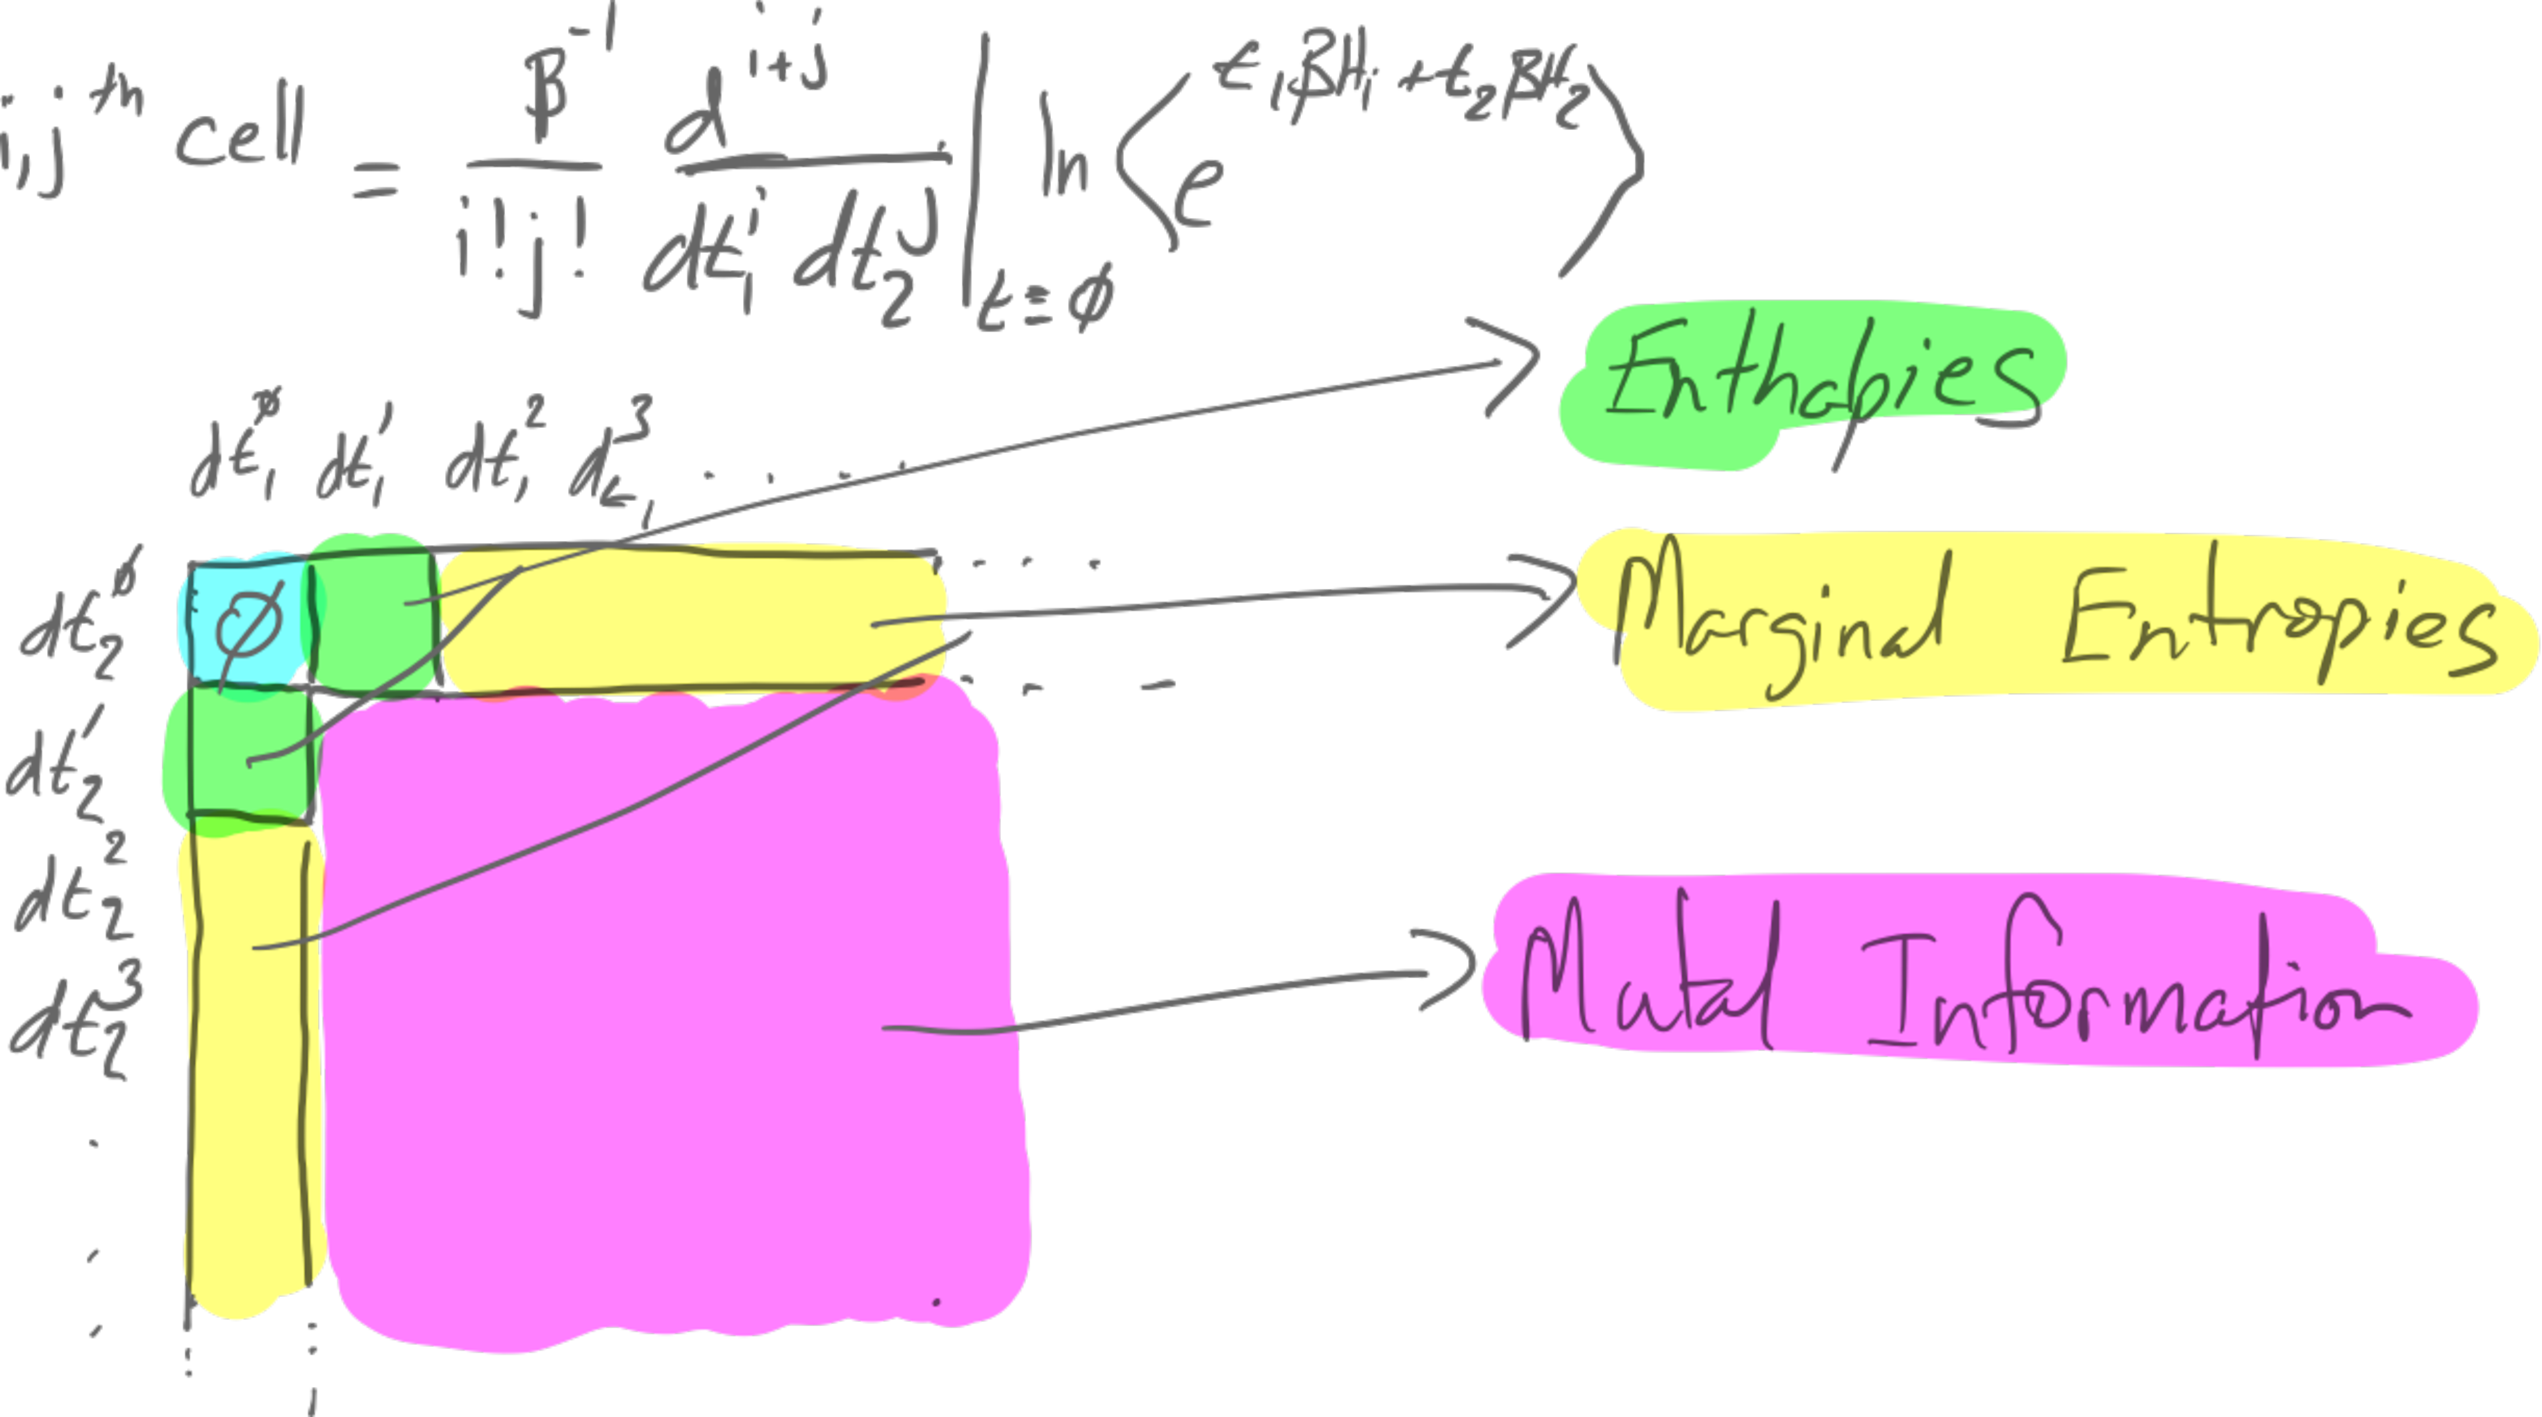
\includegraphics[width=3in]{figure2.pdf}
\caption{Graphical breakdown of free energy in terms of multivariate cumulants.}
\label{fig:2D}
\end{figure}

Eq.~\ref{eq:split} can be also be recast graphically, but this time as the sum of an infinite 2-dimensional array (Figure~\ref{fig:2D}). The $i,j=(0,0)$ cell is always zero. The $(1,0)$ and $(0,1)$ cells are the enthalpic components $\langle H_1 \rangle_\lambda$ and $\langle H_2 \rangle_\lambda$, respectively. The sum of the remaining terms is the entropic free energy. 

%\begin{figure}[htb]
%\centering
%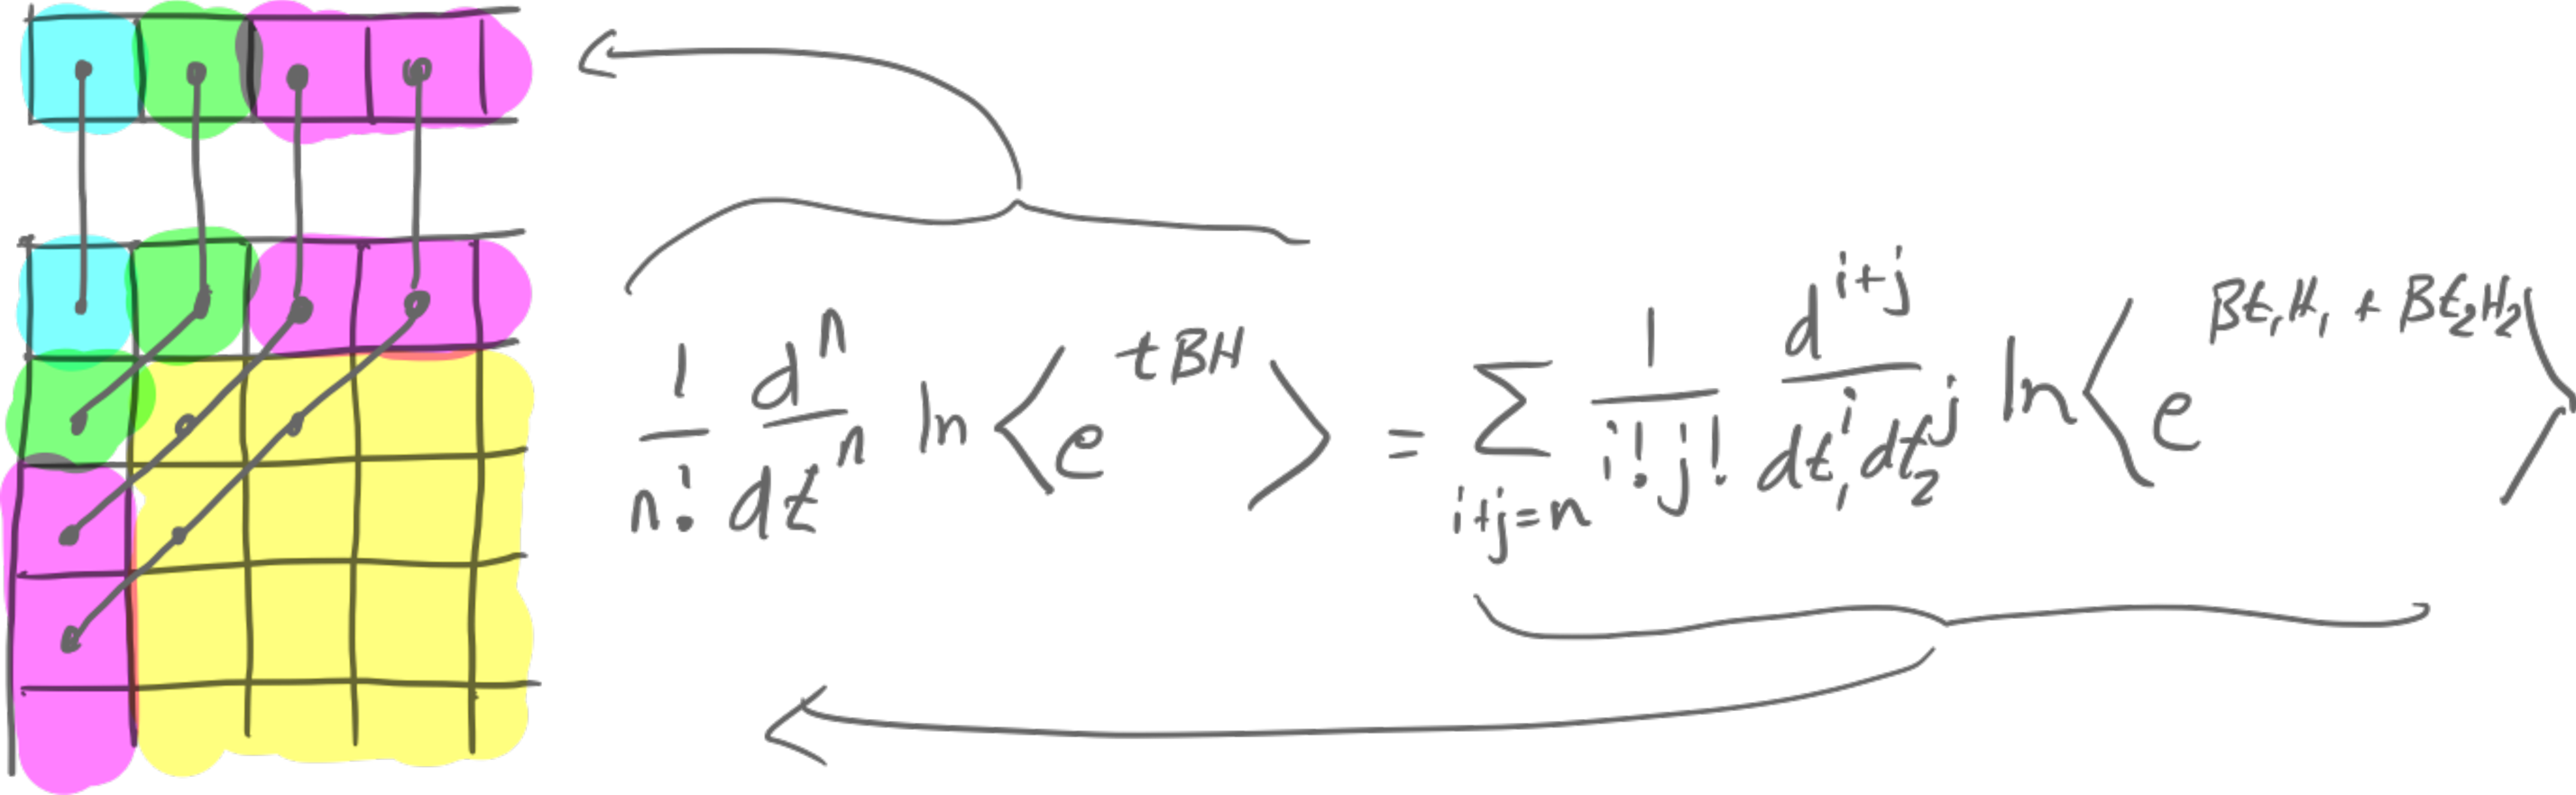
\includegraphics[width=3in]{figure3.pdf}
%\caption{The multivariate cumulants to a given order sum to the univariate cumulant of the same order.}
%\label{fig:cumsum}
%\end{figure}


The total entropy change can further be decomposed (Figure~\ref{fig:2D}) into two univariate marginal entropic contributions, $\mathcal{S}(H_1)$ and $\mathcal{S}(H_2)$, magenta region, and a bivariate joint entropic contribution, $\mathcal{S}(H_1, H_2)$, yellow region, defined as follows:
\begin{align}
\Delta \mathcal{S}(H_1) =& 
\beta^{-1} \int_0^1 \sum_{i=2}^{\infty} \frac{1}{i!}
    \left[ D_{i,j=0} K_\lambda' \right]_{t=0} d\lambda = , 
    \\ 
    \Delta \mathcal{S}(H_2) =& 
    \beta^{-1} \int_0^1 \sum_{j=2}^{\infty} \frac{1}{j!}
    \left[ D_{i=0,j}K_\lambda' \right]_{t=0} d\lambda , 
        \\ 
    \Delta \mathcal{S}(H1,H_2) =& 
    \beta^{-1} \int_0^1 \sum_{n=2}^{\infty} \sum_{\substack{i+j=n \\ i\neq0,j\neq0}} \frac{1}{i!j!}
        \left[ D_{i,j}K_\lambda' \right]_{t=0} d\lambda . 
\label{eq:mult_expansion}
\end{align}
This graphical representation is useful for visualizing free energy components that are defined later. 

This graphical decomposition extends to higher dimensions, although it becomes difficult to visualize. A three component Hamiltonian would have:
\begin{itemize}
	\item three enthalpies: $\langle H_1 \rangle_\lambda$, $\langle H_2 \rangle_\lambda$, $\langle H_3 \rangle_\lambda$,
	\item three univariate entropic contributions: $\mathcal{S}(H_1)$, $\mathcal{S}(H_2)$, $\mathcal{S}(H_3)$,
	\item three bivariate entropic contributions: $\mathcal{S}(H_1, H_2)$, $\mathcal{S}(H_1, H_3)$, $\mathcal{S}(H_2, H_3)$, 
	\item and a single trivariate entropic contribution: $\mathcal{S}(H_1, H_2, H_3)$.
\end{itemize}


%%%%%%%%%
%%%%%%%%%
%%%%%%%%%
\subsection{Free energy components can be obtained by splitting up cumulants}
%%%%%%%%%
%%%%%%%%%
%%%%%%%%%

The cumulants are state functions, so we can define path-independent free energy decompositions by splitting the cumulants between the different components. We calculate a \textbf{free energy component} $u$ as: 
\begin{align}
 A_u(\lambda) &=
	\beta^{-1} \sum_{n=1}^{\infty}
	\sum_{i+j=n}
	\frac{a_{i,j}^{(u)}}{i!j!}\left[ D_{i,j} K_\lambda\right]_{t=0},
\nonumber \\ 
\Delta \Delta A_u &= \beta^{-1} \int_0^1 \sum_{n=1}^{\infty}
	\sum_{i+j=n}
	\frac{a_{i,j}^{(u)}}{i!j!}
    	\left[ D_{i,j} K_\lambda' \right]_{t=0} d\lambda
\label{eq:Components}
\end{align}
where $u$ indexes the component, and $a_{i,j}^{(u)}$ are the \textbf{splitting coefficients}. The splitting coefficients divide each cumulant between the free energy components and are subject to $\sum_u a_{i,j}^{(u)}=1$, and therefore the components sum to the total free energy change $\sum_u \Delta \Delta A_u = \Delta A$. We next derive two useful decomposition schemes. 

We used the notation of two deltas for the free energy component $\Delta \Delta A_u$. In our first decomposition below, the free energy components do not correspond to any real free energy quantity, and a notation of $\Delta A_u$ would be just as valid as $\Delta \Delta A_u$. In our second decomposition, the free energy components do correspond to measurable free energy values and $\Delta \Delta A_u$ is the correct notation. 


%%%%%%%%%
%%%%%%%%%
\subsubsection{Thermodynamic integration components have a sensible splitting of coupled terms}
%%%%%%%%%
%%%%%%%%%

A commonly approach is to calculate free energy components directly from thermodynamic integration~\cite{NULL}, equation~\ref{eq:TI}, which suggests a natural decomposition:
\begin{equation}
\Delta \Delta  A_u =
	\int_0^1 \left\langle H_u' \right \rangle_\lambda d\lambda \nonumber\\
%\Delta\Delta A_2 =&
%	\int_0^1 \left\langle \frac{dH_2(\lambda)}{d\lambda}\right\rangle_\lambda d\lambda.    
\label{eq:naive}
\end{equation}
for $u \in \left\{1,2 \right\}$ and $\Delta A = \Delta \Delta A_1 + \Delta \Delta A_2$.  These free energy components are, in general, path-dependent. For example, in a step-wise alchemical calculation in which Hamiltonian terms $H_1$ and $H_2$ are turned on separately, the free energy components $\Delta \Delta A_1$ and $\Delta \Delta A_2$ will depend on which of these terms is turned on first. 

However, these free energy components equation~\ref{eq:naive} are indeed state functions under a large set of circumstances; i.e., when the $\lambda-$scalings of $H_1$ and $H_2$ are \textit{identical} and \textit{separable}, i.e. $H_1 (\lambda) = f(\lambda) h_1$ and  $H_2 (\lambda) = f(\lambda) h_2$
for a differentiable function $f (\lambda)$. For an alchemical path of this form, thermodynamic integration gives free energy components with the splitting coefficients 
\begin{align} 
a_{i,j}^{(1)} &= \frac{i}{i+j}, \nonumber \\ 
a_{i,j}^{(2)} &= \frac{j}{i+j}.
\label{eq:BradyCoeffs}
\end{align} 
This splits the cumulants in a sensible manner based on the contribution of each Hamiltonian component. A term $\left \langle H_1 H_2 \right \rangle_\lambda$ is evenly divided between $A_1(\lambda)$ and $ A_2(\lambda)$. Similarly, the term $\left \langle H_1^2 H_2 \right \rangle_\lambda$ is partitioned $2:1$ between $A_1(\lambda)$ and $ A_2(\lambda)$. 

This is similar to a decomposition presented in Brady and Sharp~\cite{Brady:1996gm}, which gives a special case of the above analyses.  In that work, the $\beta=0$, or non-interacting, state is taken as reference and the Hamiltonian components scale linearly in $\beta$.  Thus, their results were only postulated to be valid for free energy calculations scaled linearly from the infinite-temperature regime, and the result was shown for the first few terms but not proven in general. 

Here, we demonstrate that this decomposition is valid for a much broader class of alchemical paths (those consistent with separable and identical $\lambda$-scaling).  A proof is given in Appendix~\ref{app:IDscaling} and shows that the thermodynamic integration calculation, equation \ref{eq:naive}, gives free energy components with the above splitting coefficients, equations~\ref{eq:BradyCoeffs}. 

Therefore, path independent free energy components can be obtained directly from thermodynamic integration. However, there is still the issue of couplings among the Hamiltonian components: though the above splitting is `sensible,' the free energy components $\Delta \Delta A_u$ are not true free energies: they do not correspond to a difference in thermodynamic potential between two states, and they are not experimentally measurable. However, Karplus, Sharp, and others have argued that in many cases the couplings may be small and, therefore, these free energy components still provide useful information if interpreted carefully~\cite{Boresch:1994jj,Brady:1995dz,Boresch:1995ux,Archontis:1996ef}. For example, these free energy decompositions may be useful for identifying `hot spot' residues in, e.g., a protein-protein binding calculation.  Though they are not reliable quantitatively, they may be able to \textit{qualitatively} rank these per-residue contributions to the overall free energy.  

%%%%%%%%%
%%%%%%%%%
\subsubsection{Meaningful free energy components can be obtained from univariate and multivariate expansions}
%%%%%%%%%
%%%%%%%%%

This section contains our central results. While the previous section defined `free energy components' that are easy to calculate, they are not true free energies and they are difficult to interpret. Here, we define a new set of free energy components that are true free energies, easy to interpret, and that connect to experimental measurements.   

The free energy components are defined by the splitting coefficients
\begin{align}
a_{i,j}^{(1)} =&
	\begin{cases}
	1 &\text{if}\ i>0,  j=0 \\
	0 &\text{otherwise}
	\end{cases} \nonumber \\
a_{i,j}^{(2)} =&
	\begin{cases}
	1 &\text{if}\ i=0,  j>0  \\
	0 &\text{otherwise}
	\end{cases}  \nonumber \\
a_{i,j}^{(1,2)} =&
	\begin{cases}
	1 &\text{if}\ i>0,  j>0 \\
	0 &\text{otherwise}.
	\end{cases} \label{eq:splitCoeffsGood}
\end{align}
This decomposition has free energy components indexed by both univariate and multivariate terms, 
and these splitting coefficients would be extended to higher order terms for a Hamiltonian with three or more components. Figure~\ref{fig:good_split} shows how the cumulants are divided in this decomposition. $\Delta\Delta A_1$ contains all of the cumulants to depend only on $H_1$, $\Delta\Delta A_2$ contains all of the cumulants that depend only on $H_2$, and $\Delta\Delta A_{1,2}$ contains all of the cumulants that depend on both $H_1$ and $H_2$. 

%We will show below that $\Delta\Delta A_1$ and $\Delta\Delta A_2$ are the free energies if the corresponding Hamiltonian component is set to zero, while $\Delta\Delta A_1 + \Delta\Delta A_1 + \Delta\Delta A_{1,2}$ is the free energy if both $H_1$ and $H_2$ are set to zero.

\begin{figure}[tb]
\centering
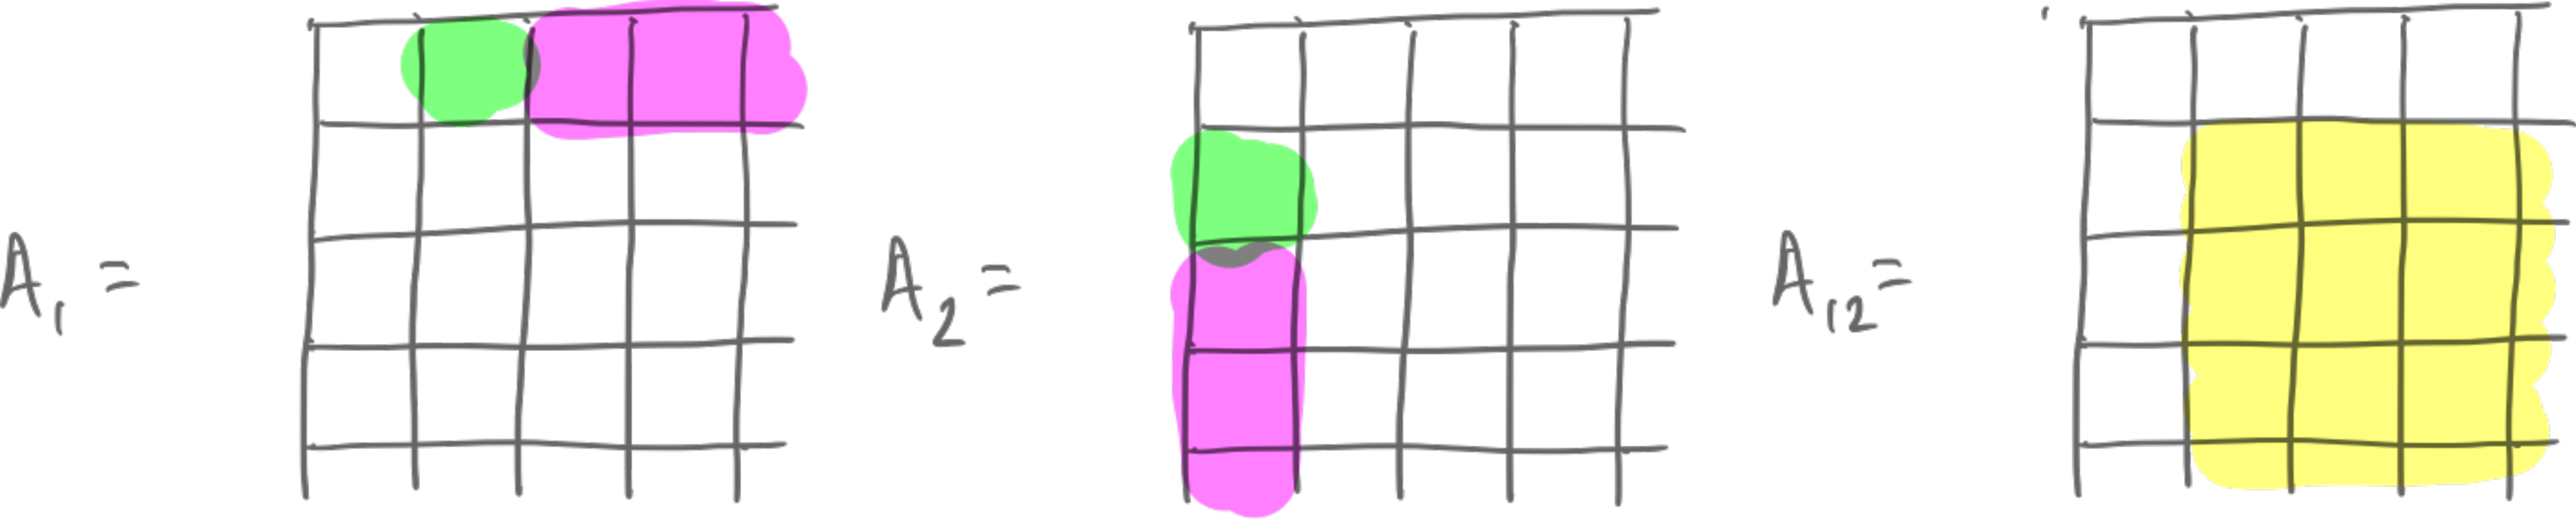
\includegraphics[width=3in]{figure5.pdf}
\caption{It is advantageous to partition joint entropic contributions into their own free energy components.}
\label{fig:good_split}
\end{figure}

This decomposition is readily interpretable and enables predictions. The free energy components are most easily written as their thermodynamic derivatives: 
\begin{align}
\frac{\partial \Delta  A_1}{\partial \lambda} =&
	\left\langle
		H_1'
	\right\rangle_\lambda +
	\left\langle
		H_2'
	\right\rangle_\lambda -
	\frac
		{\left\langle H_2' e^{\beta H_1} \right\rangle_\lambda}
		{\left\langle e^{\beta H_1} \right\rangle_\lambda} \nonumber  \\
\frac{\partial \Delta A_2}{\partial \lambda} =&
	\left\langle
		H_1'
	\right\rangle_\lambda +
	\left\langle
		H_2'
	\right\rangle_\lambda -
	\frac
		{\left\langle H_1' e^{\beta H_2} \right\rangle_\lambda}
		{\left\langle e^{\beta H_2} \right\rangle_\lambda} \nonumber \\
\frac{\partial \Delta A_{1,2}}{\partial \lambda} =&
	\frac
		{\left\langle H_2' e^{\beta H_1} \right\rangle_\lambda}
		{\left\langle e^{\beta H_1} \right\rangle_\lambda} +
	\frac
		{\left\langle H_1' e^{\beta H_2} \right\rangle_\lambda}
		{\left\langle e^{\beta H_2} \right\rangle_\lambda} -
	\left\langle
		H_1'
	\right\rangle_\lambda -
	\left\langle
		H_2'
	\right\rangle_\lambda
	\label{eq:GoodComponents}
\end{align}
A derivation is given in the next section. Here, we examine what these free energy components mean. This says that free energy component $\Delta \Delta A_1$ is equal to the total free energy less the free energy that would be obtained if $H_1$ were zero, and similarly for $\Delta \Delta A_2$. The term  $\Delta \Delta A_{1,2}$ captures the \textit{coupling} of components $1$ and $2$: the contribution of both components to the overall free energy beyond their isolated contributions. This coupling term $\Delta \Delta A_{1,2}$ is commonly measured in double mutant cycles~\cite{Cho:2014fl}.

Further intuition for these free energy components can be seen with an example. Figure~\ref{f:DoubleMutant} uses a double mutant cycle for protein-protein binding. The bottom states are two proteins separated and non-interacting, the top states correspond to the bound proteins. There are four different binding free energies corresponding to four different protein sequences: native (yellow), and with null mutations to residue A (green), to residue B (blue), and to both residues A and B (grey). In this schematic, $\Delta \Delta A_1$ is the difference between binding free energies of the native protein and the protein will a null mutant A (yellow minus green), and similarly for $\Delta \Delta A_2$ (yellow minus blue). The negative of the coupling term $\Delta \Delta A_{1,2}$ gives the non-additivity of these contributions (yellow plus grey minus green minus blue). 

The connection between $\Delta \Delta A_{1,2}$ and the double mutant cycle is easy to see for this system with two Hamiltonian components, where the free energy difference with both null mutations (grey) is zero since $\lambda$ does not affect the Hamiltonian in either state.  Though it's not obvious, $\Delta \Delta A_{1,2}$ also matches the double mutant experiment in the more general case, when there are more than two Hamiltonian components scaled by $\lambda$ and this reference free energy difference does not disappear; see Appendix~\ref{app:3components}. 

\warning{The description and figure are temporary. We can change both to match whatever example we like, protein folding, ligand binding, etc.}

\begin{figure}
 \centering
  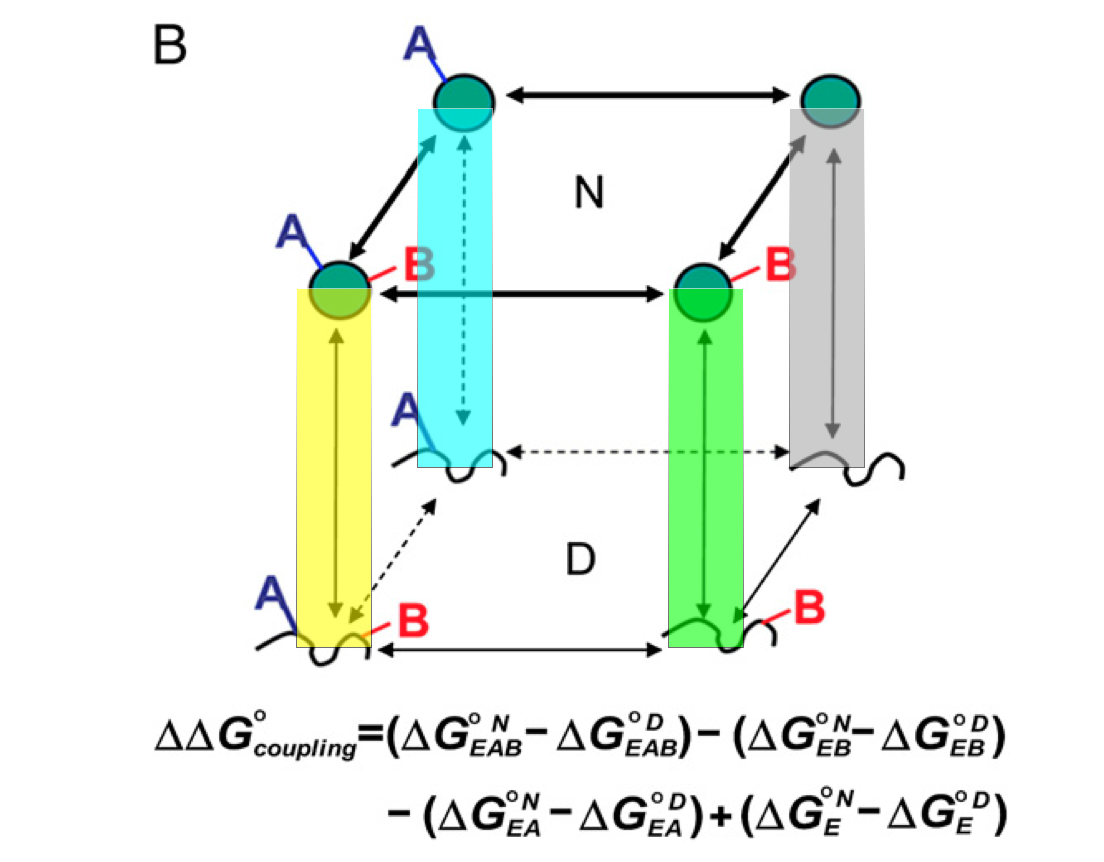
\includegraphics[width=8.6cm]{doubleMutantColors.png}
\caption{\label{f:DoubleMutant}{ A double mutant cycle. Though the figure, taken from Ref.~\cite{Cho:2014fl}, is for protein folding, I'm using it as an example for protein-protein binding, where the bottom square corresponds to separated states and the top corresponds to bound states.  }}
\end{figure}


%%%%%%%%%
%%%%%%%%%
\subsubsection{Derivation of the free energy components and how they can be calculated}
\label{sec:ComponentDerivation}
%%%%%%%%%
%%%%%%%%%

To derive equations~\ref{eq:GoodComponents}, we start from the definition of a free energy component, equation \ref{eq:Components}, and rearrange terms into a better form. First, evaluating the derivative of the cumulant generating function, equation \ref{eq:cGenMulti}, with respect to $\lambda$ gives:
\begin{equation}
K_\lambda' = 
	\beta \left[
		t_1 \left\langle H_1' \right\rangle_{\vec t,\lambda} -
    	\left\langle H_1' \right\rangle_{\vec t,\lambda} +
	    t_2 \left\langle H_2' \right\rangle_{\vec t,\lambda} -
    	\left\langle H_2' \right\rangle_{\vec t,\lambda}
    \right], 
    \label{eq:kprime}
\end{equation}
where we have dropped terms with no $\vec t$-dependence that will disappear in subsequent steps, and the notation $\langle X \rangle_{\vec t, \lambda}$ means
\begin{equation}
\langle X \rangle_{\vec t, \lambda}  =
	\frac
    	{\int X(x, \lambda) 
        	\exp\left[
        		\beta(t_1-1)H_1(\lambda) +
            \beta(t_2-1)H_2(\lambda)
        \right] dx
        }
    	{\int
        	\exp\left[
            \beta(t_1-1)H_1(\lambda) +
            \beta(t_2-1)H_2(\lambda)
        \right] dx
        }.
\end{equation}

The general form of $D_{i,j}K'$ is:
\begin{equation}
[D_{i,j}K_\lambda']_{\vec t=0} =
	\beta\left[
		i \phi_{i-1, j}^{(1)}(\lambda) -
    	\phi_{i,j}^{(1)}(\lambda) +
    	j \phi_{i, j-1}^{(2)}(\lambda) -
    	\phi_{i,j}^{(2)}(\lambda)
    \right],
\label{eq:deriv}
\end{equation}
where we have introduced the notation
\begin{equation}
\phi_{i,j}^{(v)}(\lambda) =
	\left[ D_{i,j} \left\langle
    	H_v'
    \right\rangle_{\vec t, \lambda} \right]_{\vec t=0}.
    \label{eq:phi}
\end{equation}
Equation~\ref{eq:deriv} is not obvious but can be easily shown with induction, see Appendix~\ref{app:Derivation}. 


Each term $\phi_{i,j}^{(1)}$ can be produced in two different ways, from $D_{i,j}K'$ or $D_{i+1,j}K'$. Similarly, each $\phi_{i,j}^{(2)}$ can be produced from $D_{i,j}K'$ or $D_{i,j+1}K'$. Regrouping similar terms, we can rewrite Eq.~\ref{eq:split} as: 
\begin{equation}
\Delta\Delta {A_u}=
	\int_0^1 \left(
        a_{1,0}^{(u)}\left\langle H_1' \right\rangle_{\lambda} +
        a_{0,1}^{(u)}\left\langle H_2' \right\rangle_{\lambda} +
        \psi_1^{(u)}(\lambda) +
        \psi_2^{(u)}(\lambda)
    \right) d\lambda,
\label{eq:dA_expansion}
\end{equation}
with
\begin{align}
\psi_1^{(u)}(\lambda) &=
	\sum_{n=1}^{\infty}
    \sum_{i+j=n}
        \frac{\phi_{i,j}^{(1)}}{i!j!}
        \left(
            {a_{i+1,j}^{(u)}} -
            {a_{i,j}^{(u)}}
        \right) \label{eq:psi1}\\
\psi_2^{(u)}(\lambda) &=
	\sum_{n=1}^{\infty}
    \sum_{i+j=n}
        \frac{\phi_{i,j}^{(2)}}{i!j!}
        \left(
            a_{i,j+1}^{(u)} -
            a_{i,j}^{(u)}
      	\right)\label{eq:psi2}.
\end{align}
Substituting the splitting coefficients, equation~\ref{eq:splitCoeffsGood}, into equation~\ref{eq:dA_expansion} gives:
\begin{align}
\frac{\partial \Delta A_1}{\partial\lambda} =& 
	\left\langle
		 H_1'
	\right\rangle_\lambda -
	\phi_{1,0}^{(2)} -
	\frac{1}{2} \phi_{2,0}^{(2)} -
	\frac{1}{6} \phi_{3,0}^{(2)} - \ldots \nonumber\\
	=&
	\left\langle
		H_1'
	\right\rangle_\lambda -
	\sum_{n=1}^{\infty} \frac{1}{n!} \phi_{n,0}^{(2)}.
\label{eq:almost_taylor}
\end{align}
If we define $f(t)$ as:
\begin{equation}
f(t) = \frac
	{\int H_2' e^{\beta(t-1) H_1 - \beta H_2} dx}
	{\int e^{\beta(t-1) H_1 - \beta H_2} dx},
\end{equation}
we see that the sum in Eq.~\ref{eq:almost_taylor} is almost the series of $f(t=1)$ expanded around $t=0$. Adding and subtracting the missing zeroth order term gives:
\begin{align}
\frac{\partial \Delta A_1}{\partial \lambda} =&
	\left\langle
		H_1'
	\right\rangle_\lambda +
	f(0) -
	\left(
		\sum_{n=1}^{\infty} \frac{1}{n!}
		\left[ \frac{\partial^n}{\partial t^n} f(t) \right]_{t=0}
		+ f(0)
	\right)\nonumber\\
=&
	\left\langle
		H_1'
	\right\rangle_\lambda +
	\left\langle
		H_2'
	\right\rangle_\lambda -
	\frac
		{\int H_2' e^{-\beta H_2} dx}
		{\int e^{-\beta H_2} dx} \nonumber \\
=&
	\left\langle
		H_1'
	\right\rangle_\lambda +
	\left\langle
		H_2'
	\right\rangle_\lambda -
	\left\langle
		H_2'
	\right\rangle_{\lambda, H_1=0} \nonumber \\
=&
	\left\langle
		H_1'
	\right\rangle_\lambda +
	\left\langle
		H_2'
	\right\rangle_\lambda -
	\frac
		{\left\langle H_2' e^{\beta H_1} \right\rangle_\lambda}
		{\left\langle e^{\beta H_1} \right\rangle_\lambda}
	\label{eq:same_ensemble}
\end{align}
The final two lines express the third and final term as an average over an ensemble where $H_1$ is zero. 
Repeating this calcuation for $\Delta \Delta A_2$ and $\Delta \Delta A_{1,2}$ gives the free energy components as presented in equations~\ref{eq:GoodComponents}. 

For a system with $N$ total Hamiltonian terms (e.g., $N$ total residues is a protein-protein binding calculation), there are three ways to calculate the $N$ free energy components: 
\begin{enumerate}
	\item Perform one traditional free energy calculation for each component ($N$ total free energy calculations). Accurate, but expensive.
	\item Perform a single binding free energy calculation and calculate the exact free energy components from the exponential form, equation~\ref{eq:same_ensemble}. This is exact, but the exponential average will be very noisy, as in free energies calculated directly from the Zwanzig relationship.
	\item Perform a single binding free energy calculation and estimate each free energy component from the cumulant expansion, equation~\ref{eq:almost_taylor}, truncated to some order. This is approximate, but less noisy. 
\end{enumerate}
In the results section, we compare these three calculations. 


\subsection{Spatial vs other decompositions}

This section will explain how spatial decompositions, e.g. residue or functional group, are better. Something like electrostatics and LJ is a problematic decomposition, because thees terms share the same dof and so energies are going to be highly coupled. This leads to non-negligible higher-order cumulants that are going to be hard to estimate and split. For spatial decompositions, only terms for nearby residues are going to be strongly coupled. This means that any errors are spatially localized, so there might be some "smearing" between nearby residues.

\section{Numerical Results}


\section{Conclusions}


%%%%%%%%
%%%%%%%%
\clearpage

%%%%%%%%
%%%%%%%%
%%%%%%%%
\section*{Random bits that need to find a home}
%%%%%%%%
%%%%%%%%
%%%%%%%%
\subsection*{We can compute entropies...}

We're talking about the univariate, i.e. not components, total free energy in this section. The first cumulant is the enthalpy. The sum of all of the higher order cumulants is the entropic free energy.
\begin{equation}
-T \Delta S = \beta^{-1} \sum_{n=2}^\infty \frac{1}{n!}
	\Bigg[ 
		\frac{d^n}{dt^n}
		\ln \langle e^{t\beta H} \rangle
	\Bigg]_{t=0}.
\end{equation}

Following a similar procedure as before, we can differentiate with respect to $\lambda$:
\begin{equation}
-T\frac{d\Delta S}{d\lambda} = \beta^{-1} \sum_{n=2}^\infty \frac{1}{n!}
	\Bigg[ 
		\frac{d^n}{dt^n}
		\frac{d}{d\lambda} \ln \langle e^{t \beta H} \rangle
	\Bigg]_{t=0}.
\end{equation}
Next, we have:
\begin{equation}
\frac{d}{d\lambda} \langle e^{t \beta H} \rangle =
\beta \left[
	t \langle H' \rangle_{t, \lambda} - \langle H' \rangle_{t, \lambda}
\right],
\end{equation}
where the $\langle \cdot \rangle_{t,\lambda}$ notation has a similar meaning to previous sections.

The general form of $D_n K'$ is:
\begin{equation}
[D_n K_\lambda']_{t=0} =
	\beta\left[
		n \phi_{n-1}(\lambda) -
    	\phi_n(\lambda)
    \right],
\end{equation}
where
\begin{equation}
\phi_n(\lambda) =
	\left[ D_n \left\langle
    	H'
    \right\rangle_{t, \lambda} \right]_{t=0}.
\end{equation}
As before, each term $\phi_n$ can be produced in two different ways, from $D_n K'$ or $D_{n+1} K'$. So, for $n=2\ldots\infty$, nearly all of the terms will be paired up, but there will be a single unpaired first-order term:
\begin{align}
-T \Delta S = \int_0^1
	\Bigg[ 
		\langle H' H \rangle - \langle H' \rangle \langle H \rangle
	\Bigg] d\lambda
\end{align}
Note, that I might have the sign backwards.

This needs a better explanation, but it follows from the same logic used in other sections.

Does this even go in this paper, or do we try to write it up separately. I haven't tried to use this formula. We would need to see how it compares to the two other common ways to estimate entropy changes: (1) temperature dependence of free energy, (2) estimating enthalpy based on average energies at the endpoints, then using $-T \Delta S = \Delta G - \Delta H$.

%%%%%%%%
%%%%%%%%
\subsection*{What do the cumulants mean?}
%%%%%%%%
%%%%%%%%

Getting to Eq.~\ref{eq:same_ensemble} was a complicated way to figure out what the components mean. Instead, we can proceed as follows, which might be clearer. We start with one of the cumulants where $H_2$ is zero:
\begin{align}
\Bigg[ D_i \ln \langle e^{t_1 H_1} \rangle_{H_2=0} \Bigg]_{t_1=0} =&
	\Bigg[ D_i \ln \frac{\langle e^{t_1 H_1} e^{H_2} \rangle}{\langle e^{H_2} \rangle} \Bigg]_{t_1=0} \\
	= &
		\Bigg[ D_i \ln \langle e^{t_1 H_1} e^{H_2} \rangle \Bigg]_{t_1=0}  -
		\Bigg[ D_i \ln {\langle e^{H_2} \rangle} \Bigg]_{t_1=0} \\
	= &
		\Bigg[ D_i \ln \langle e^{t_1 H_1} e^{H_2} \rangle \Bigg]_{t_1=0}.
\end{align}
We can then introduce $t_2$, expand around $t_2=0$ and evaluate at $t_2=1$, which gives:
\begin{align}
\Bigg[ D_i \ln \langle e^{t_1 H_1} e^{H_2} \rangle \Bigg]_{t_1=0} =&
	\Bigg[ D_{i,0} \sum_{j=0}^\infty \frac{1}{j!} \Bigg[
		D_{0,j} \ln \langle e^{t_1 H_1} e^{H_2} \rangle
	\Bigg]_{t_2=0}
\Bigg]_{t_1=0} \\
=&
\sum_{j=0}^\infty \frac{1}{j!}
\Bigg[
	D_{i,j} \ln \langle e^{t_1 H_1} e^{t_2 H_2} \rangle
\Bigg]_{t_1=t_2=0}.
\end{align}

This notation needs to be cleaned up, but we've shown that each cumulant from the ensemble where $H_2=0$ is the sum of the corresponding rows in the case where $H_2$ is ``active''. From this, it's easy to deduce the meaning of our $A_1$ and $A_2$ components.




%%%%%%%%
%%%%%%%%
\subsection*{Good decompositions are readily interpretable and make predictions.}
%%%%%%%%
%%%%%%%%
\warning{I cut this section from the main text but am leaving it here for now....}

Provided the splitting coefficients are valid, that is $\sum_u a_{i,j}^{(u)}=1$, no decomposition is more ``correct'' than any other. However, some decompositions are not useful, as they are difficult to interpret and provide little or no predictive power (Figure~\ref{fig:bad_split}).

\begin{figure}[tb]
\centering
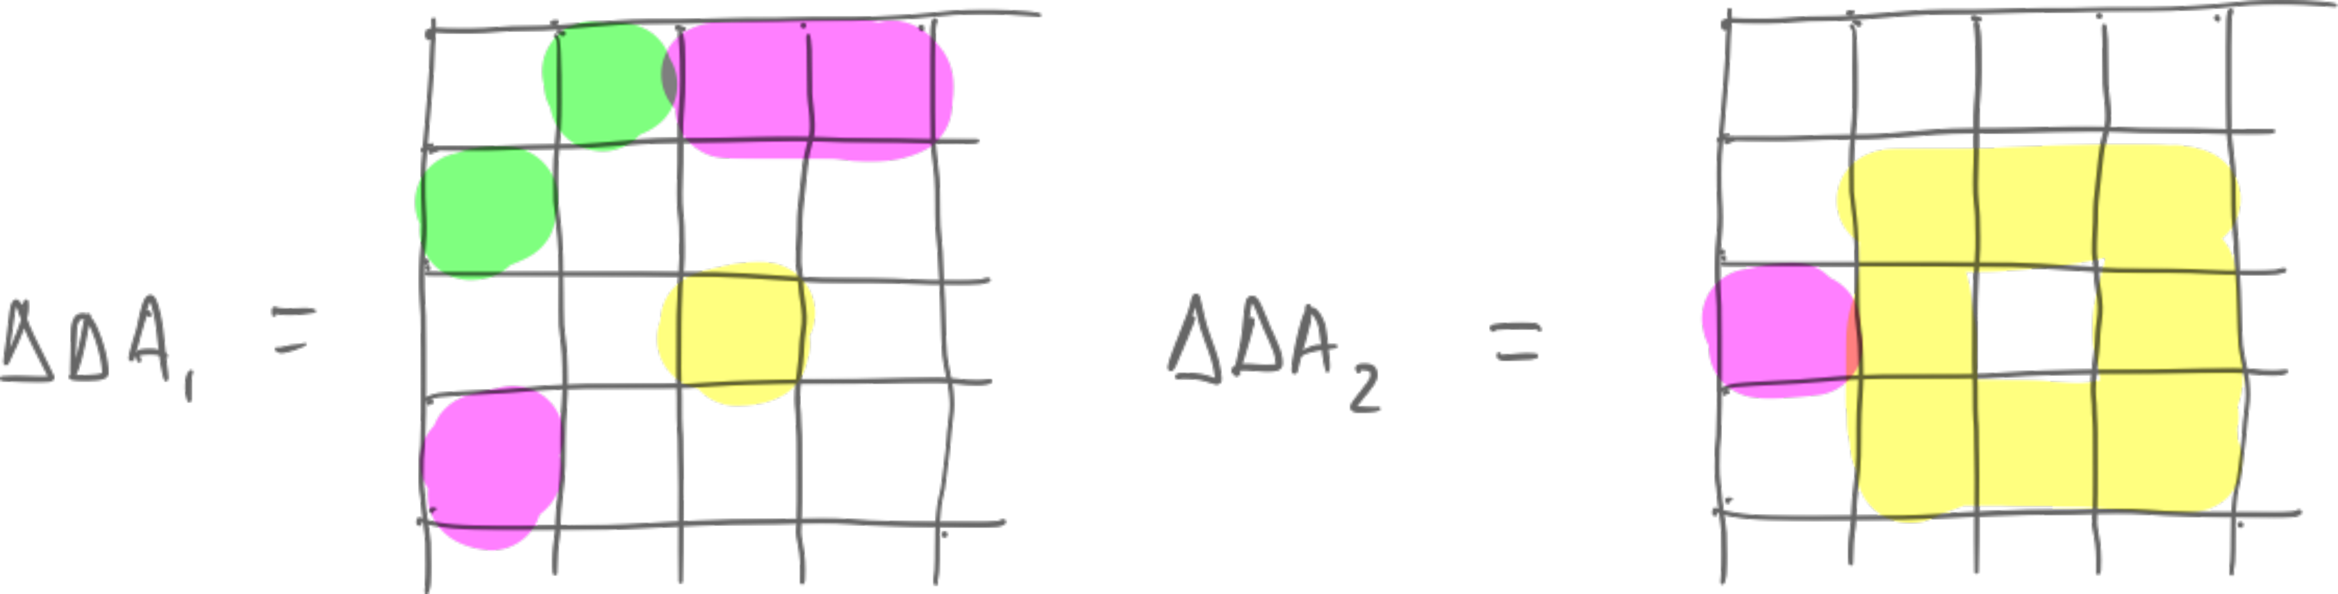
\includegraphics[width=3in]{figure6.pdf}
\caption{An example of a decomposition that is difficult to interpret and makes no useful predictions.}
\label{fig:bad_split}
\end{figure}

\begin{figure}[tb]
\centering
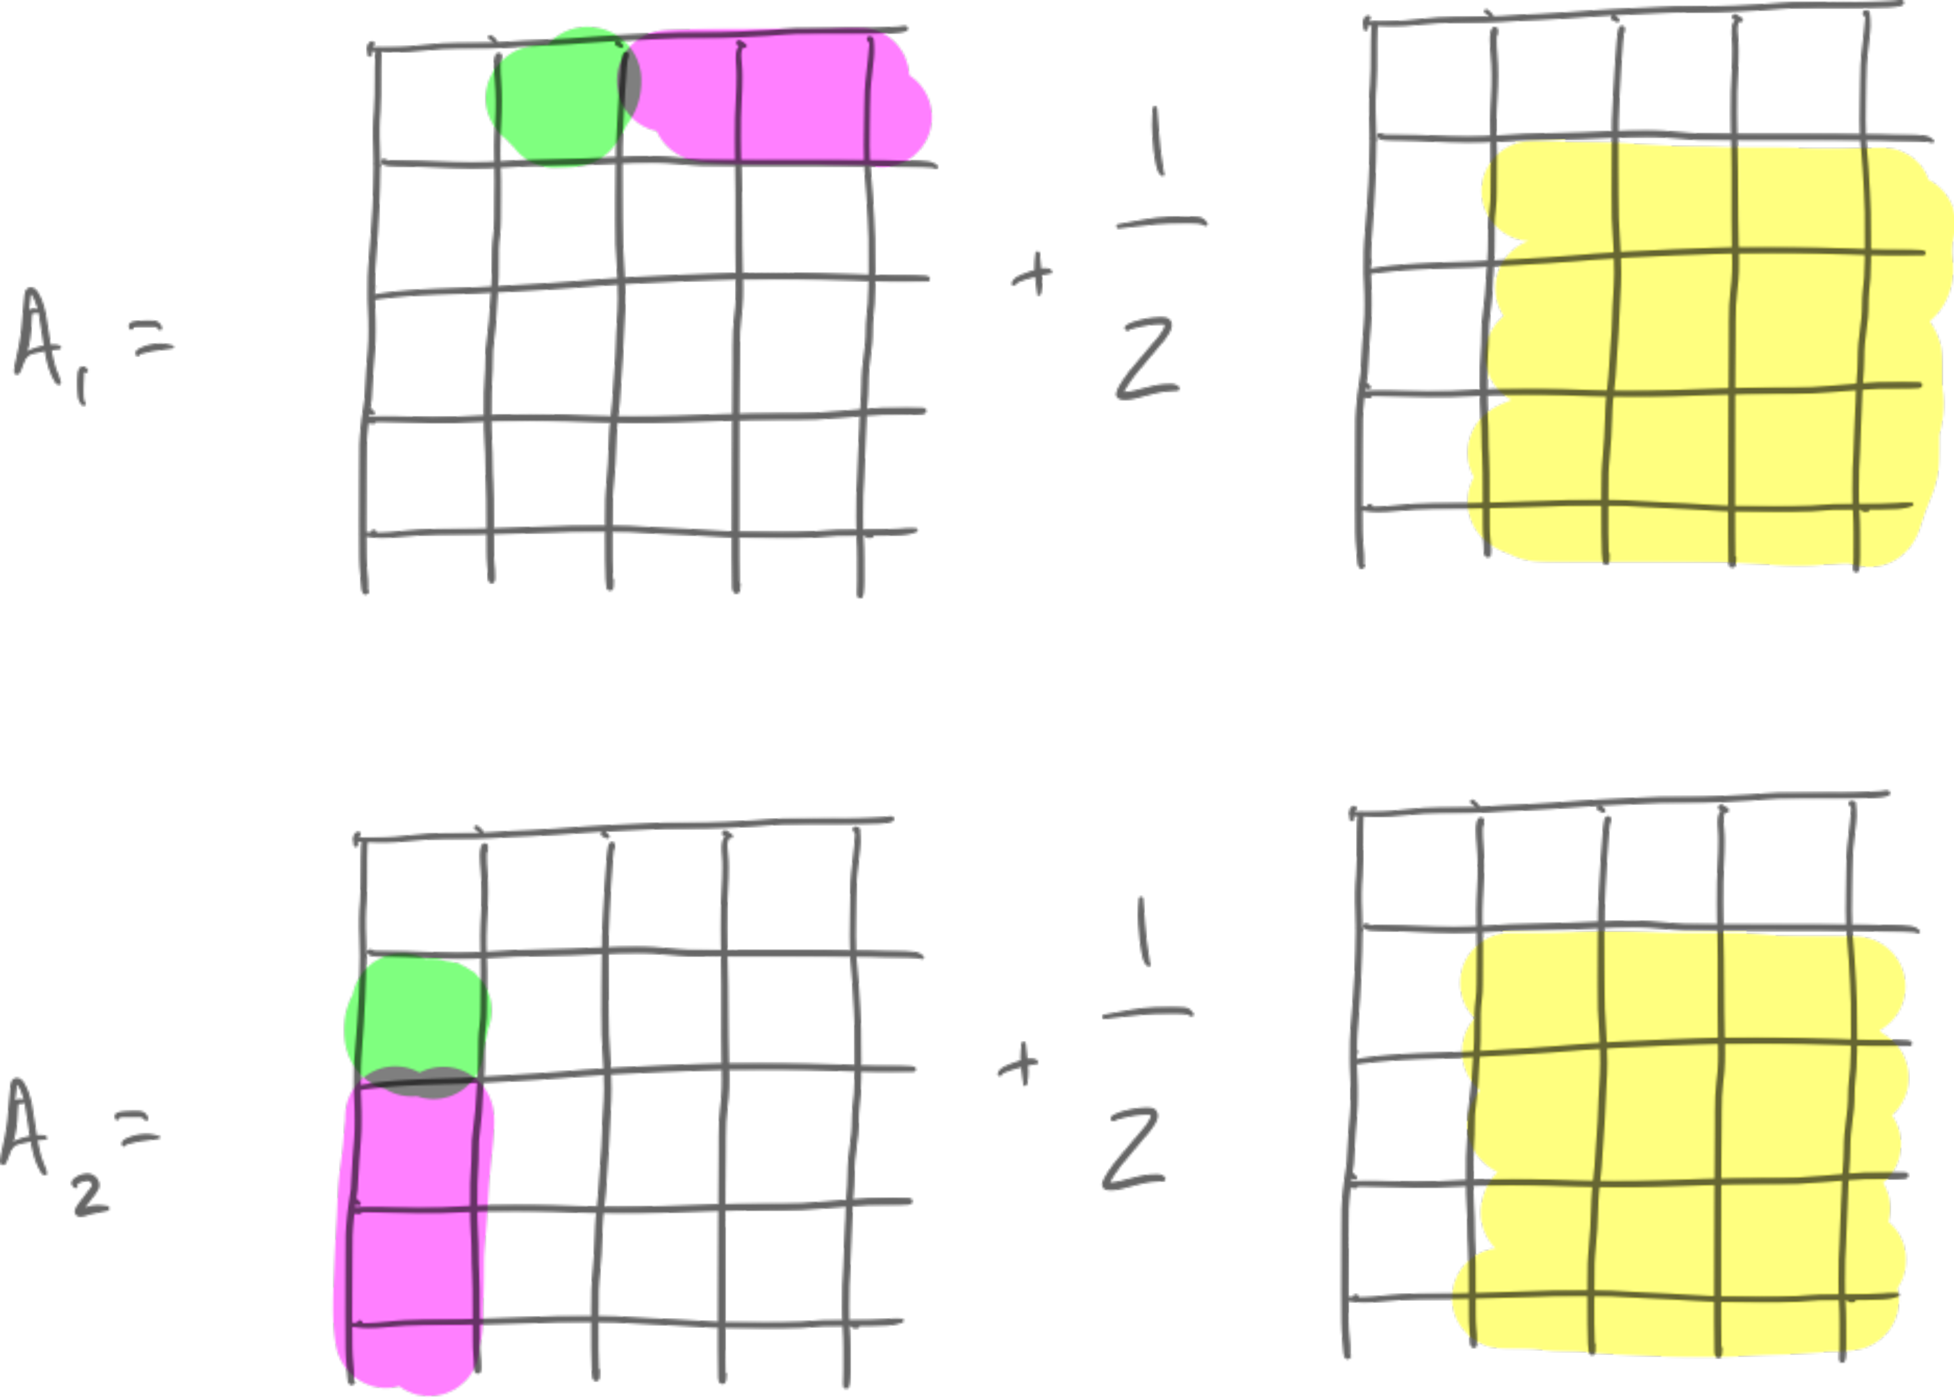
\includegraphics[width=3in]{figure4.pdf}
\caption{An example of a decomposition that is easy to interpret, but where predictions are difficult to make.}
\label{fig:ok_split}
\end{figure}

Some decompositions are more readily interpretable, e.g. Figure~\ref{fig:ok_split}. This splitting decomposes the cumulants in a obvious way, with half of each joint cumulant split between the two components. However, this decompositions does not allow us to make predictions. For example, what would the free energy be if $H_1$ was set to zero? This decomposition does not allow us to address this question.


Figure~\ref{fig:good_split} shows an example of the most useful type of decomposition. In this decomposition, $\Delta\Delta A_1$ contains all of the cumulants to depend only on $H_1$, $\Delta\Delta A_2$ contains all of the cumulants that depend only on $H_2$, and $\Delta\Delta A_{1,2}$ contains all of the cumulants that depend on both $H_1$ and $H_2$. This decomposition is readily interpretable, as each component has a clear meaning. Furthermore, this decompositions enables predictions. We will show below that $\Delta\Delta A_1$ and $\Delta\Delta A_2$ are the free energies if the corresponding Hamiltonian component is set to zero, while $\Delta\Delta A_1 + \Delta\Delta A_1 + \Delta\Delta A_{1,2}$ is the free energy if both $H_1$ and $H_2$ are set to zero.

We need to come up with consistent notation throughout. I propose $\mathcal{A}_i$ for single-component terms, $\mathcal{C}_{ij}$ for coupling terms, and $\mathcal{A}_{i,j} = \mathcal{A}_i + \mathcal{A}_j + \mathcal{C}_{i,j}$.



%%%%%%%%
%%%%%%%%
\subsection*{The path-dependence of free energy decompositions can be partially eliminated by performing a correction to finite order.}
%%%%%%%%
%%%%%%%%
\warning{I cut this section from the main text but am leaving it here for now....}

Consider the sum of terms due to $\psi_1$:
\begin{align*}
\sum_u \psi_1^{(u)} =&
	\sum_{n=1}^{\infty}
    \sum_{i+j=n}
        \frac{\phi_{i,j}^{(1)}}{i!j!}
        \left(
        		\sum_u a_{i+1,j}^{(u)} -
        		\sum_u a_{i,j}^{(u)}
        \right) = 0,
\end{align*}
where the second equality holds because each set of splitting coefficients sums to unity. A similar result holds for the terms due to $\psi_2$.

We can view each order $n$ of Eqs.~\ref{eq:psi1} and \ref{eq:psi2} as a correction towards a particular path-independent splitting. Each order of correction leaves the total free energy invariant, but shifts some free energy between the components. Thus, the path-dependence can be partially corrected by truncating Eqs.~\ref{eq:psi1} and \ref{eq:psi2} at finite order without affecting the total free energy.


%%%%%%%%
%%%%%%%%
%%%%%%%%
\section*{Appendices}
\begin{appendices}
%%%%%%%%
%%%%%%%%
%%%%%%%%
\section{The joint cumulants capture the statistical dependence of Hamiltonian components.}
\label{app:jointCumulants}

The mixed partial derivatives with respect to $\vec t$ capture the statistical dependence of Hamiltonian components to a given order. For example, the second order $\kappa_{0,1,1}$ term is simply the covariance between $H_1$ and $H_2$:
\begin{align}
\kappa_{0, 1, 1} = [D_{0, 1, 1} K_\lambda]_{\vec t=0} =&
	\beta^2 \left[
    	\left\langle H_1 H_2 \right\rangle_\lambda -
		\left\langle H_1 \right\rangle_\lambda 
		\left\langle H_2 \right\rangle_\lambda
    \right] \nonumber\\
    =&
    \beta^2 \mathrm{Cov}(H_1,H_2).              
\end{align}
This cumulant the difference between the actual average value of the product of $H_1$ and $H_2$ compared to that expected if $H_1$ and $H_2$ were statistically independent.

Similarly, the third order cumulant, $\kappa_{1,1,1}$, captures the difference between the average product of $H_0$, $H_1$, and $H_2$ compared to what is expected if they were statistically independent:
\begin{alignat}{3}
\MoveEqLeft[3] [D_{1, 1, 1} K_\lambda]_{\vec t=0}\notag\\
&= \beta^3[ &&
\left\langle H_0 H_1 H_2 \right\rangle_\lambda -
\left\langle H_0 H_1 \right\rangle_\lambda
	\left\langle H_2 \right\rangle_\lambda -
\left\langle H_0 H_2 \right\rangle_\lambda
	\left\langle H_1 \right\rangle_\lambda - \notag\\
&&& \left\langle H_1 H_2 \right\rangle_\lambda
	\left\langle H_0 \right\rangle_\lambda +
2 \left\langle H_0 \right\rangle_\lambda
	\left\langle H_1 \right\rangle_\lambda
	\left\langle H_2 \right\rangle_\lambda]\notag\\
&= \beta^3[ &&
	\left\langle H_0 H_1 H_2 \right\rangle_\lambda -
	\mathrm{Cov}(H_0,H_1) \left\langle H_2 \right\rangle_\lambda -
	\mathrm{Cov}(H_0,H_2) \left\langle H_1 \right\rangle_\lambda -\\
	&&& \mathrm{Cov}(H_1,H_2) \left\langle H_0 \right\rangle_\lambda -
	\left\langle H_0 \right\rangle_\lambda
		\left\langle H_1 \right\rangle_\lambda
		\left\langle H_2 \right\rangle_\lambda]        
\end{alignat}
This cumulant accounts for all of the ways that there can be independence, where either all three variables being independent, or where two of the variables are dependent, but the third is independent.

Expressions for higher-order cumulants rapidly become more complex, but they all capture the same...


%%%%%%%%
%%%%%%%%
\section{Cancellation of spectator components}
\label{app:Spectator}
%%%%%%%%
%%%%%%%%
\warning{Show that spectator components cancel in equation~\ref{eq:split}.}


%%%%%%%%
%%%%%%%%
\section{Identical scaling leads to a natural splitting where most terms cancel}
\label{app:IDscaling}
%%%%%%%%
%%%%%%%%

Consider the case where the $\lambda$-dependence is an identical scaling, $H(\lambda) = f(\lambda)h_1 + f(\lambda)h_2$. In these circumstances,
\begin{equation*}
\frac{\partial}{\partial t_1}
	\langle H_2' \rangle_{\vec t, \lambda} = 
\frac{\partial}{\partial t_2}
	\langle H_1' \rangle_{\vec t, \lambda},
\end{equation*}
which implies
\begin{equation}
\phi_{i,j}^{(2)} = \phi_{i-1,j+1}^{(1)}, 
\label{eq:separable}
\end{equation}
using the notation introduced in Section~\ref{sec:ComponentDerivation}. 
Substitution of Eq.~\ref{eq:separable} into Eq.~\ref{eq:deriv} gives
\begin{align}
[D_{i,j}K_\lambda']_{\vec t=0} &=
	\beta\left[
		i \phi_{i-1, j}^{(1)}(\lambda) -
    	\phi_{i,j}^{(1)}(\lambda) +
    	j \phi_{i-1, j}^{(1)}(\lambda) -
    	\phi_{i-1,j+1}^{(1)}(\lambda)
    \right] \nonumber \\
    &=
	\beta\left[
		(i + j)\phi_{i-1, j}^{(1)}(\lambda) -
    	\phi_{i,j}^{(1)}(\lambda) -
    	\phi_{i-1,j+1}^{(1)}(\lambda)
    \right].
\end{align}
Each term $\phi_{i,j}^{(1)}$ can be produced in three different ways, from $D_{i,j}K'$, $D_{i+1,j}K'$, or $D_{i+1,j-1}K'$. Grouping of similar terms gives
\begin{equation}
\Delta\Delta A_u =
	\int_0^1 \left(
        a_{1,0}^{(u)}f'(\lambda)
        \left\langle h_1 \right\rangle +
        a_{0,1}^{(u)}f'(\lambda)
        \left\langle h_2 \right\rangle +
        \sigma(\lambda)
    \right) d\lambda,
\end{equation}
with
\begin{align}
\sigma(\lambda) &=
	\sum_{n=1}^{\infty}
    \sum_{i+j=n}
        \frac
        	{\phi_{i,j}^{(1)}}
            {i!j!}
        \left(
            \frac
                {(i+j+1)a_{i+1,j}^{(u)}}
                {i+1} -
            a_{i,j}^{(u)} -
           	\frac
            	{j a_{i+1,j-1}^{(u)}}
                {i+1}
		\right).
\label{eq:cancel}
\end{align}
Cancellation of the bracketed terms in Eq.~\ref{eq:cancel} requires
\begin{equation}
\frac
	{(i+j+1)a_{i+1,j}^{(u)}}
	{i+1} -
a_{i,j}^{(u)} -
\frac
	{j a_{i+1,j-1}^{(u)}}
	{i+1}
= 0.
\end{equation}
Under the constraints $a_{1,0}^{(1)} = 1$ and $a_{0,1}^{(2)} = 1$, the solution is
\begin{align}
a_{i,j}^{(1)} &= \frac{i}{i+j} \nonumber\\
a_{i,j}^{(2)} &= \frac{j}{i+j} \nonumber\\
\label{eq:splitting}
\end{align}
leading to
\begin{equation}
\begin{split}
\Delta\Delta A_1 &= 
	\int_0^1 f'(\lambda)
    \langle h_1 \rangle 
    d\lambda \\
\Delta\Delta A_2 &= 
	\int_0^1 f'(\lambda)
    \langle h_2 \rangle
    d\lambda.
\end{split}
\end{equation}
Thus, in the case of identical scaling, the na\"ive scaling given by Eq.~\ref{eq:naive} results in a well-defined splitting of the cumulants. This result is similar to that in previous work.

%%%%%%%%
%%%%%%%%
\section{The double mutant cycle with a three component Hamiltonian}
\label{app:3components}
%%%%%%%%
%%%%%%%%
To rigorously connect our free energy components to a double mutant experiment, we need to derive these components for a Hamiltonian in which the reference state $H_0$ also has a $\lambda-$dependence: $H(x, \lambda) = H_0 (x) + H_1(x, \lambda) + H_2(x, \lambda)$, since this will be the case for most experiments or simulations.  In this section we use an expanded version of the notation introduced in Section~\ref{sec:ComponentDerivation}: 
\begin{equation}
\phi_{i,j,k}^{(v)}(\lambda) =
	\left[ D_{i,j,k} \left\langle
    	H_v'
    \right\rangle_{\vec t, \lambda} \right]_{\vec t=0}.
    \label{eq3:phi}
\end{equation}
(analogous to equation~\ref{eq:phi}, for three components) and $D_{i,j,k}$ means $\partial^{i+j+k} /(\partial t_0^i \partial t_1^j \partial t_2^k)$. 

 Starting from equation~\ref{eq:dA_expansion} and rewriting with all three components: 
\begin{align}
\Delta\Delta A_u &=
	\int_0^1 \left(
	a_{1,0,0}^{(u)}\left\langle H_0' \right\rangle_{\lambda} +
        a_{0,1,0}^{(u)}\left\langle H_1' \right\rangle_{\lambda} +
        a_{0,0,1}^{(u)}\left\langle H_2' \right\rangle_{\lambda} 
\right. \nonumber \\ & \qquad \qquad \left. + 
        \psi_0^{(u)}(\lambda) +
        \psi_1^{(u)}(\lambda) +
        \psi_2^{(u)}(\lambda)
    \right) d\lambda,
\label{eq3:dA_expansion}
\end{align}
with
\begin{align}
\psi_0^{(u)}(\lambda) &=
	\sum_{n=1}^{\infty}
    \sum_{i+j+k=n}
        \frac{\phi_{i,j,k}^{(0)}}{i!j!k!}
        \left(
            {a_{i+1,j,k}^{(u)}} -
            {a_{i,j,k}^{(u)}}
        \right) \label{eq3:psi0}\\
\psi_1^{(u)}(\lambda) &=
	\sum_{n=1}^{\infty}
    \sum_{i+j+k=n}
        \frac{\phi_{i,j,k}^{(1)}}{i!j!,k!}
        \left(
            {a_{i,j+1,k}^{(u)}} -
            {a_{i,j,k}^{(u)}}
        \right) \label{eq3:psi1}\\
\psi_2^{(u)}(\lambda) &=
	\sum_{n=1}^{\infty}
    \sum_{i+j+k=n}
        \frac{\phi_{i,j,k}^{(2)}}{i!j!k!}
        \left(
            a_{i,j,k+1}^{(u)} -
            a_{i,j,k}^{(u)}
      	\right)\label{eq3:psi2}.
\end{align}

This system has 7 total free energy components, $u \in \left\{ 0;1;2;0,1;0,2;1,2;0,1,2\right\}$. The splitting coefficients are: 
\begin{align}
a_{i,j,k}^{(1)} =&
	\begin{cases}
	1 &\text{if}\ i=0,  j>0,k=0 \\
	0 &\text{otherwise}
	\end{cases} \nonumber \\
a_{i,j,k}^{(1,2)} =&
	\begin{cases}
	1 &\text{if}\ i=0,  j>0,k>0 \\
	0 &\text{otherwise}.
	\end{cases} \nonumber \\ 
a_{i,j,k}^{(0,1,2)} =&
	\begin{cases}
	1 &\text{if}\ i>0,  j>0,k >0 \\
	0 &\text{otherwise}.
	\end{cases} 
\label{eq3:splitCoeffsGood}
\end{align}
where, for simplicity, we have only written three representative coefficients, $u \in \left\{ 1;1,2;0,1,2 \right\}$, one each of a one-body, two-body, and three-body component. 


Substituting the splitting coefficients, equation~\ref{eq3:splitCoeffsGood}, into equation~\ref{eq3:dA_expansion} gives:
\begin{align}
\frac{\partial \Delta A_1}{\partial\lambda} =& 
	\left\langle
		 H_1'
	\right\rangle_\lambda -
	\phi_{0,1,0}^{(0)} -
	\frac{1}{2} \phi_{0,2,0}^{(0)} -
	\frac{1}{6} \phi_{0,3,0}^{(0)} - \ldots \nonumber\\
	& \qquad \qquad 
	 -
	\phi_{0,1,0}^{(2)} -
	\frac{1}{2} \phi_{0,2,0}^{(2)} -
	\frac{1}{6} \phi_{0,3,0}^{(2)} - \ldots \nonumber\\
	=&
	\left\langle
		H_1'
	\right\rangle_\lambda -
	\sum_{n=1}^{\infty} \frac{1}{n!} \left( \phi_{0,n,0}^{(0)} + \phi_{0,n,0}^{(2)} \right). 
\label{eq3:almost_taylor}
\end{align}
If we define $f(t)$ as:
\begin{equation}
f(t) = \frac
	{\int (H_0'+H_2') e^{-\beta H_0 + \beta(t-1) H_1 - \beta H_2} dx}
	{\int e^{-\beta H_0 + \beta(t-1) H_1 - \beta H_2} dx},
\end{equation}
we see that the sum in Eq.~\ref{eq:almost_taylor} is almost the series of $f(t=1)$ expanded around $t=0$. Adding and subtracting the missing zeroth order term gives:
\begin{align}
\frac{\partial \Delta A_1}{\partial \lambda} =&
	\left\langle
		H_1'
	\right\rangle_\lambda +
	f(0) -
	\left(
		\sum_{n=1}^{\infty} \frac{1}{n!}
		\left[ \frac{\partial^n}{\partial t^n} f(t) \right]_{t=0}
		+ f(0)
	\right)\nonumber\\
=&
	\left\langle
		H_0'
	\right\rangle_\lambda +
	\left\langle
		H_1'
	\right\rangle_\lambda +
	\left\langle
		H_2'
	\right\rangle_\lambda -
	\frac
		{\left\langle (H_0' + H_2' )e^{\beta H_1} \right\rangle_\lambda}
		{\left\langle e^{\beta H_1} \right\rangle_\lambda} . 
	\label{eq3:same_ensemble}
\end{align}
As before, this equation shows that $\Delta \Delta A_1$ is the total free energy less the free energy were component $H_1$ set to zero. 

We can similarly evaluate $\Delta \Delta A_{1,2}$ to find
\begin{align}
\frac{\partial \Delta A_{1,2}}{\partial\lambda} =& 
	- \sum_{n=1}^{\infty}
	\sum_{\substack{j+k=n \\ j>0,k>0}}
	  \frac{\phi_{0jk}^{(0)}}{j!k!}
	+  \sum_{k=1}^{\infty}  \frac{\phi_{00k}^{(1)}}{k!}
	+  \sum_{j=1}^{\infty}  \frac{\phi_{0j0}^{(2)}}{j!}
\nonumber \\ =& 
	- \sum_{n=1}^{\infty}
	\sum_{j+k=n}
	  \frac{\phi_{0jk}^{(0)}}{j!k!}
	+  \sum_{k=1}^{\infty}  \frac{\phi_{00k}^{(0)}+\phi_{00k}^{(1)}}{k!}
	+  \sum_{j=1}^{\infty}  \frac{\phi_{0j0}^{(0)}+\phi_{0j0}^{(2)}}{j!}
\nonumber \\ =& 
	-\left \langle H_0'\right \rangle_{\lambda} - \sum_{n=1}^{\infty} \sum_{j+k=n} \frac{\phi_{0jk}^{(0)}}{j!k!}
\nonumber \\ & 
	+  \left \langle H_0'\right \rangle_{\lambda}+\left \langle H_1'\right \rangle_{\lambda}+\sum_{k=1}^{\infty}  \frac{\phi_{00k}^{(0)}+\phi_{00k}^{(1)}}{k!}
\nonumber \\ & 
	+ \left \langle H_0'\right \rangle_{\lambda}+\left \langle H_2'\right \rangle_{\lambda}+  \sum_{j=1}^{\infty}  \frac{\phi_{0j0}^{(0)}+\phi_{0j0}^{(2)}}{j!}
\nonumber \\ &
	-\left \langle H_0'\right \rangle_{\lambda}-\left \langle H_1'\right \rangle_{\lambda}-\left \langle H_2'\right \rangle_{\lambda}
\nonumber \\ =& 
	-\left \langle H_0'\right \rangle_{\lambda}-\left \langle H_1'\right \rangle_{\lambda}-\left \langle H_2'\right \rangle_{\lambda}
	+\frac
		{\left\langle (H_0' + H_1' )e^{\beta H_2} \right\rangle_\lambda}
		{\left\langle e^{\beta H_2} \right\rangle_\lambda}
\nonumber \\ &
	+\frac
		{\left\langle (H_0' + H_2' )e^{\beta H_1} \right\rangle_\lambda}
		{\left\langle e^{\beta H_1} \right\rangle_\lambda}
	-\frac
		{\left\langle H_0' e^{\beta (H_1+H_2)} \right\rangle_\lambda}
		{\left\langle e^{\beta (H_1+H_2)} \right\rangle_\lambda}		
\label{eq3:almost_taylor12}
\end{align}
This confirms that $\Delta \Delta A_{1,2}$ matches the negative of the coupling free energy commonly measured in double mutant cycles: $\Delta \Delta A_{1,2}$ captures the \textit{coupling} of components $1$ and $2$: the contribution of both components to the overall free energy beyond their isolated contributions. For the free energy cycle shown in Figure~\ref{f:DoubleMutant}: \warning{In the notation of that figure, with G replaced by A}
\begin{align}
\Delta \Delta A_{1,2} =& 
	-\left(\Delta A_{EAB}^N- \Delta A_{EAB}^D \right) + \left(\Delta A_{EB}^N- \Delta A_{EB}^D \right)
\nonumber \\ & 
	+ \left(\Delta A_{EA}^N- \Delta A_{EA}^D \right) - \left(\Delta A_{E}^N- \Delta A_{E}^D \right)
\nonumber \\  = &
	-\Delta \Delta A_{\text{coupling}}
\end{align}


%%%%%%%%
%%%%%%%%
\section{Derivation of equation~\ref{eq:deriv}}
\label{app:Derivation}
%%%%%%%%
%%%%%%%%
\warning{I kept getting confused by this equation every time I hadn't looked at the manuscript in a few days, so I decided to add more detail.}

Here we derive equation~\ref{eq:deriv}. The form of this equation, before it is evaluated at $\vec{t}=0$, is:
\begin{align}
D_{i,j}K_\lambda'&=
	\beta\left[
		i D_{i-1,j} \left \langle H_1' \right \rangle_{\vec t, \lambda}  + \left(t_1-1\right) D_{i,j} \left \langle H_1' \right \rangle_{\vec t, \lambda} 
	\right. \nonumber \\ & \qquad \left. 
		+ j D_{i,j-1} \left \langle H_2' \right \rangle_{\vec t, \lambda}   + \left(t_2-1\right) D_{i,j} \left \langle H_2' \right \rangle_{\vec t, \lambda}  \right]
\label{eq:derivGen}
\end{align}
We first derive this equation~\ref{eq:derivGen} by induction, then evaluate it at $\vec{t}=0$ to arrive at equation~\ref{eq:deriv}. 
	
 First, the base cases. Taking the derivatives of $K_{\lambda}'$ in equation~\ref{eq:kprime}: 
\begin{align}
D_{1,0} K_{\lambda}' & = 
	\beta \left[ \left \langle H_1' \right \rangle_{\vec t, \lambda}  + \left(t_1-1\right) D_{1,0} \left \langle H_1' \right \rangle_{\vec t, \lambda}  + \left(t_2-1\right) D_{1,0} \left \langle H_2' \right \rangle_{\vec t, \lambda}  \right], 
\label{eq:D10} \\ 
D_{0,1} K_{\lambda}' & = 
	 \beta  \left[ \left(t_1-1\right) D_{0,1} \left \langle H_1' \right \rangle_{\vec t, \lambda}  + \left \langle H_2' \right \rangle_{\vec t, \lambda}  + \left(t_2-1\right) D_{0,1} \left \langle H_2' \right \rangle_{\vec t, \lambda}   \right], 
\label{eq:D01} \\ 
D_{1,1} K_{\lambda}' & = 
 	\beta \left[ D_{0,1} \left \langle H_1' \right \rangle_{\vec t, \lambda}  + \left(t_1-1\right) D_{1,1} \left \langle H_1' \right \rangle_{\vec t, \lambda} 
	\right. \nonumber \\ & \qquad \left. 
	+ D_{1,0} \left \langle H_2' \right \rangle_{\vec t, \lambda}  + \left(t_2-1\right) D_{1,1} \left \langle H_2' \right \rangle_{\vec t, \lambda}  \right], 
\label{eq:D11}
\end{align}
where equation~\ref{eq:D11}, found either by taking the derivative of equation~\ref{eq:D10} with respect to $t_2$ or by taking the derivative of equation~\ref{eq:D01} with respect to $t_1$, confirms the base case of equation~\ref{eq:derivGen}. 

Next, the induction step. We take the partial derivative of  equation~\ref{eq:derivGen} with respect to $t_1$ to obtain:
\begin{align}
D_{i+1,j}K_\lambda &= \beta \left[ 
	i  D_{i,j} \left \langle H_1' \right \rangle_{\vec t, \lambda}  + D_{i,j} \left \langle H_1' \right \rangle_{\vec t, \lambda}  + \left(t_1-1\right) D_{i+1,j} \left \langle H_1' \right \rangle_{\vec t, \lambda} 
\right. \nonumber \\ & \qquad \left. 
	+ j D_{i+1,j-1} \left \langle H_2' \right \rangle_{\vec t, \lambda}   + \left(t_2-1\right) D_{i,j+1} \left \langle H_2' \right \rangle_{\vec t, \lambda} 
	\right]. 
\label{eq:Di1j}
\end{align}
Substituting $i+1,j$ into equation~\ref{eq:derivGen} matches this equation~\ref{eq:Di1j}, confirming the induction step. Evaluating equation~\ref{eq:derivGen} at $\vec{t}=0$ then gives equation~\ref{eq:deriv}. 



\end{appendices}

\bibliographystyle{unsrt}
\bibliography{DecompRefs}

\end{document}